\chapter{Introduction of PitchApp}
\chapterauthor{by Boglarka Lehoczki}

\section{The Value PitchApp Provides for Businesses}

PitchApp is intended to be a platform to help employees find the required organizational support to turn their ideas from inception to reality. The goal of our web-application is, thus, to facilitate the launching of new projects. By making project ideas of colleagues easier and faster visible to management, PitchApp encourages employees to contribute more actively to the success of the company at which they work. In this way, PitchApp helps to achieve higher degrees of intrapreneurship, which leads to business growth. Using our application will bring companies ahead of the game, in terms of innovation and
employee engagement, as well as make big firms more competitive and flexible, thus more
profitable. Hence, “fast innovators take leadership positions in their industries” \parencite{SH90}.

\section{Characteristics of PitchApp}

PitchApp is a dynamic, single-page web-application with database connection that we developed to enhance employee engagement and proactivity by connecting the employees’ ideas to even the highest levels of executives. Managers with budgets and resources for projects (i.e. potential future sponsors) can browse between different project ideas, which are posted by the employees. Distinct types of ideas are sorted into groups like HR, Procurement, R\&D etc., which facilitates searching among them. Then managers can offer their resources for the realization of a project idea, which they find valuable. Employees are also able to view the pitches posted by other colleagues in between their organization to avoid the sharing of redundant ideas. PitchApp is planned to be able to serve more large organizations at the same time and to be provided as a Software as a Service. PitchApp includes a user and session management system, which allows secure login and logout functionalities. It differentiates between public area, i.e. our landing page, and member area with two type of users, idea owners and idea sponsors.

\break

The table above shows how PitchApp fulfills the given project requirements.

\begin{center}
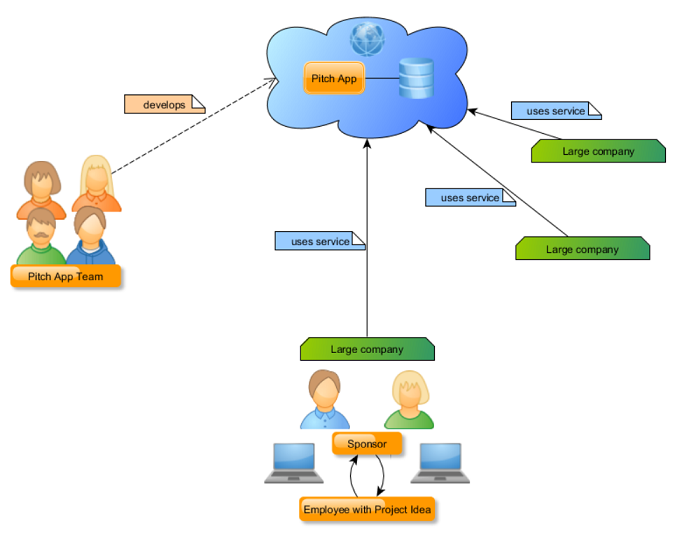
\includegraphics{pitchapp_saas.png}
\end{center}

The figure above presents the general characteristics of PitchApp.

\begin{table}[]
	\resizebox{\textwidth}{!}{%
		\begin{tabular}{@{}lll@{}}
			\toprule
			Requirement                                                                           & Status & Technology                \\ \midrule
			Log in / Log out (differentiation between public section and member area)             & done   & Okta                      \\
			User management                                                                       & done   & Okta                      \\
			Session management                                                                    & done   & Okta                      \\
			Application linked to a database                                                      & done   & PostgreSQL                \\
			Dynamic content                                                                       & done   & React single-page web-app \\
			Not high complexity, but challenging/latest technologies & done   & See above                 \\ \bottomrule
		\end{tabular}%
	}
\end{table}



\chapter{Architecture}
\chapterauthor{by Boglarka Lehoczki}

\section{Client-Server Architecture}

PitchApp implements a classic client-server architecture. More specifically, PitchApp is a web-application and has a 3-tier architecture. The three tiers are the user interface (UI), the application server and the database server. In such an architecture, the UI runs in a web-browser like Google Chrome or Mozilla Firefox. The UI communicates with the application server through HTTP requests and responses, as the application server also implements web-server functionalities. The application server itself acts as a client of the database server \parencite[p.~80]{MT17}. The interaction between these two servers can be based on different protocols or database connectivities, like JDBC for JAVA or ODBC for ABAP. In the case of PitchApp, this communication is solved by a Hasura GraphQL Engine, which auto-generates queries as part of the GraphQL schema from our Postgres schema model \parencite{Hasura}. The application server fetches the needed data from the database server, which returns it to the client in its reply. The process described above is shown by the following figure \parencite[p.~80]{MT17}.

\begin{center}
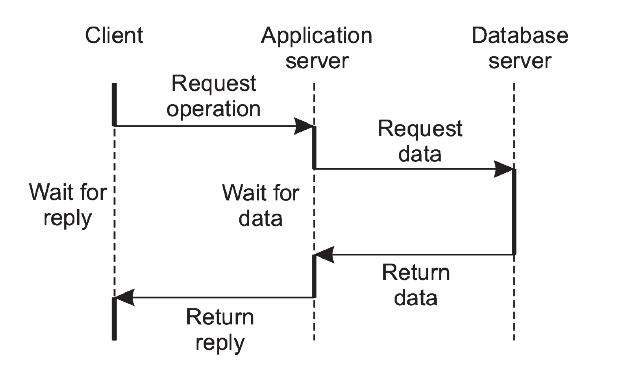
\includegraphics{3tiers_gen.png}
\end{center}

\break

The following figure gives a generalized example on how the tiers interact with each other when a user wants to see only those pitches, which were created by him or herself. This figure is based on another one from the book Distributed Systems \parencite[p.~61]{MT17}.

\begin{center}
	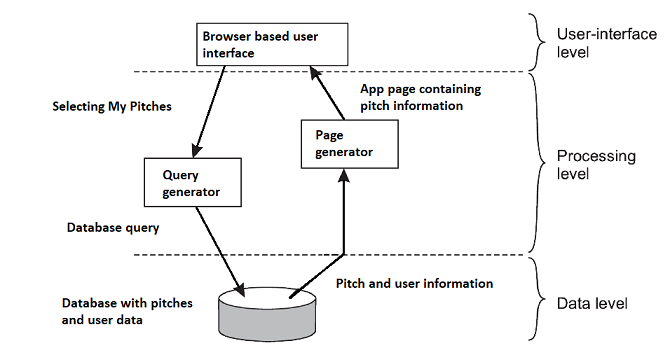
\includegraphics{3tiers_architecture.png}
\end{center}

Developing a web-application was a given requirement and it has several advantages. In comparison to a native application (with 2-tier architecture), the user do not have to install any additional application to its local machine, because the web-application runs in a browser. From this also follows, that if in the future we e.g. change the UI, users do not have to download updates onto their local machine. An other benefit of web-applications is that they are easier to scale and the different tiers can be scaled separately based on the use case. From the viewpoint of PitchApp this is particularly important, as our application has to be able to serve a large number of users from our customer companies.

\break

\section{Technologies used for each Tier of PitchApp's Architecture}

We selected state-of-the-art technologies to implement PitchApp. To develop a dynamic single-page web-application, React was used. With Reactstrap, we were able to create a responsive and neat-looking UI. Including an Okta modul to our web-application helped us to provide our users a secure authentication, user- and session management system. Our back-end is a Hasura GraphQL Engine which communicates easily with a PostgreSQL database. The following figure shows the architecture of PitchApp.

\begin{center}
	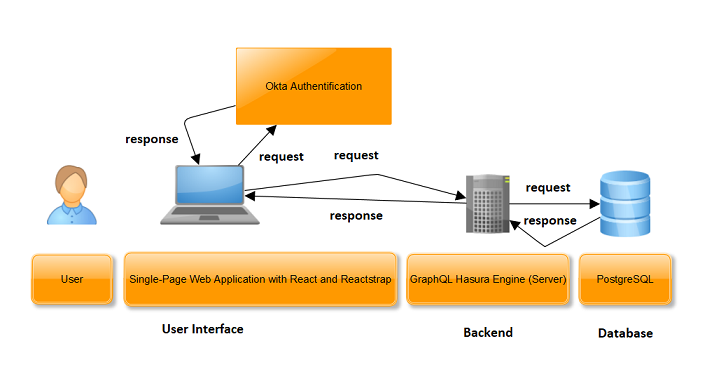
\includegraphics{pitchapp_architecture.png}
\end{center}


\chapter{Technologies used for Implementation}
\section{React and Reactstrap}
\chapterauthor{by Boglarka Lehoczki}

The client side of our web-application, PitchApp, was implemented by using React and Reactstrap, which is built on Bootstrap. The following figure presents how the relevant client side technologies are built on top of each other.

\begin{center}
	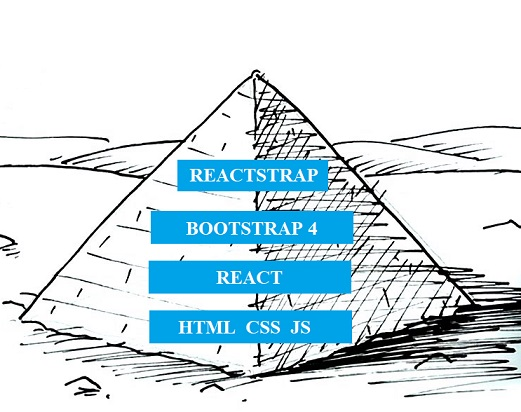
\includegraphics{pyramid.jpg}
\end{center}  

The basis of these web-technologies is the classical web-development trio of Hypertext Markup Language (HTML), Cascading Style Sheets (CSS) and JavaScript (JS). The .html, .css and .js files, which are executed to display the UI on the client side by the web-browser, are delivered by the web-server. HTML is used to describe the content of a web-page. CSS defines the design and layout of this content. JS is commonly used to implement further functionality and to build a dynamic web-page. JS is also called a scripting language, because it determines the way the content of the received web-page is parsed into the Document Object Model (DOM). In this way, the content of the received page can be manipulated. PitchApp was developed to fulfill the requirements of dynamic web-development and, through this, to achieve a higher level of user interactivity.

To achieve this, we used React, which is a JS library and helps to create web-based graphical UIs \parencite{React}. React works with JSX \parencite{JSX}, which can be described as a syntax extension for JS and combines characteristics of HTML and JS. As the basis of our web-application, a React App was created \parencite{Reactstrap}. The reasons, why we decided to implement PitchApp using React, are based on the general characteristics of React.

With this library, it is easy to develop interactive web-applications. React with JSX, just as JS, is used to access and manipulate the DOM of a web-page or web-application. It is done in the index.html file, where the root from <div id="root"></div> is replaced by all the content of PitchApp, which are to be found in the source folder (src directory) and collected into one component <App/>. In the index.js file, the React DOM is mapped to the root with the following code: ReactDOM.render(<App />, document.getElementById('root'));.

React is declarative and component-based. This means, that the presented UI elements are programmed as a component and can be used and rendered when needed to the UI. The following example shows code snippets from Home.js, which is the landing page of PitchApp and HomeJumbotron.js, which is a jumbotron component of PitchApp displayed on the publicly available landing page.

\begin{center}
	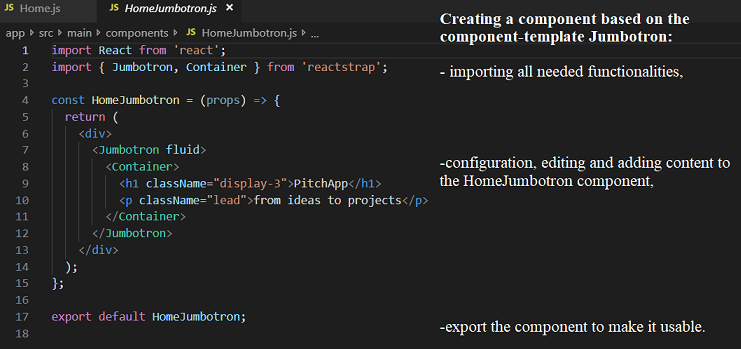
\includegraphics{home_jumbotron.png}
\end{center} 

\begin{center}
	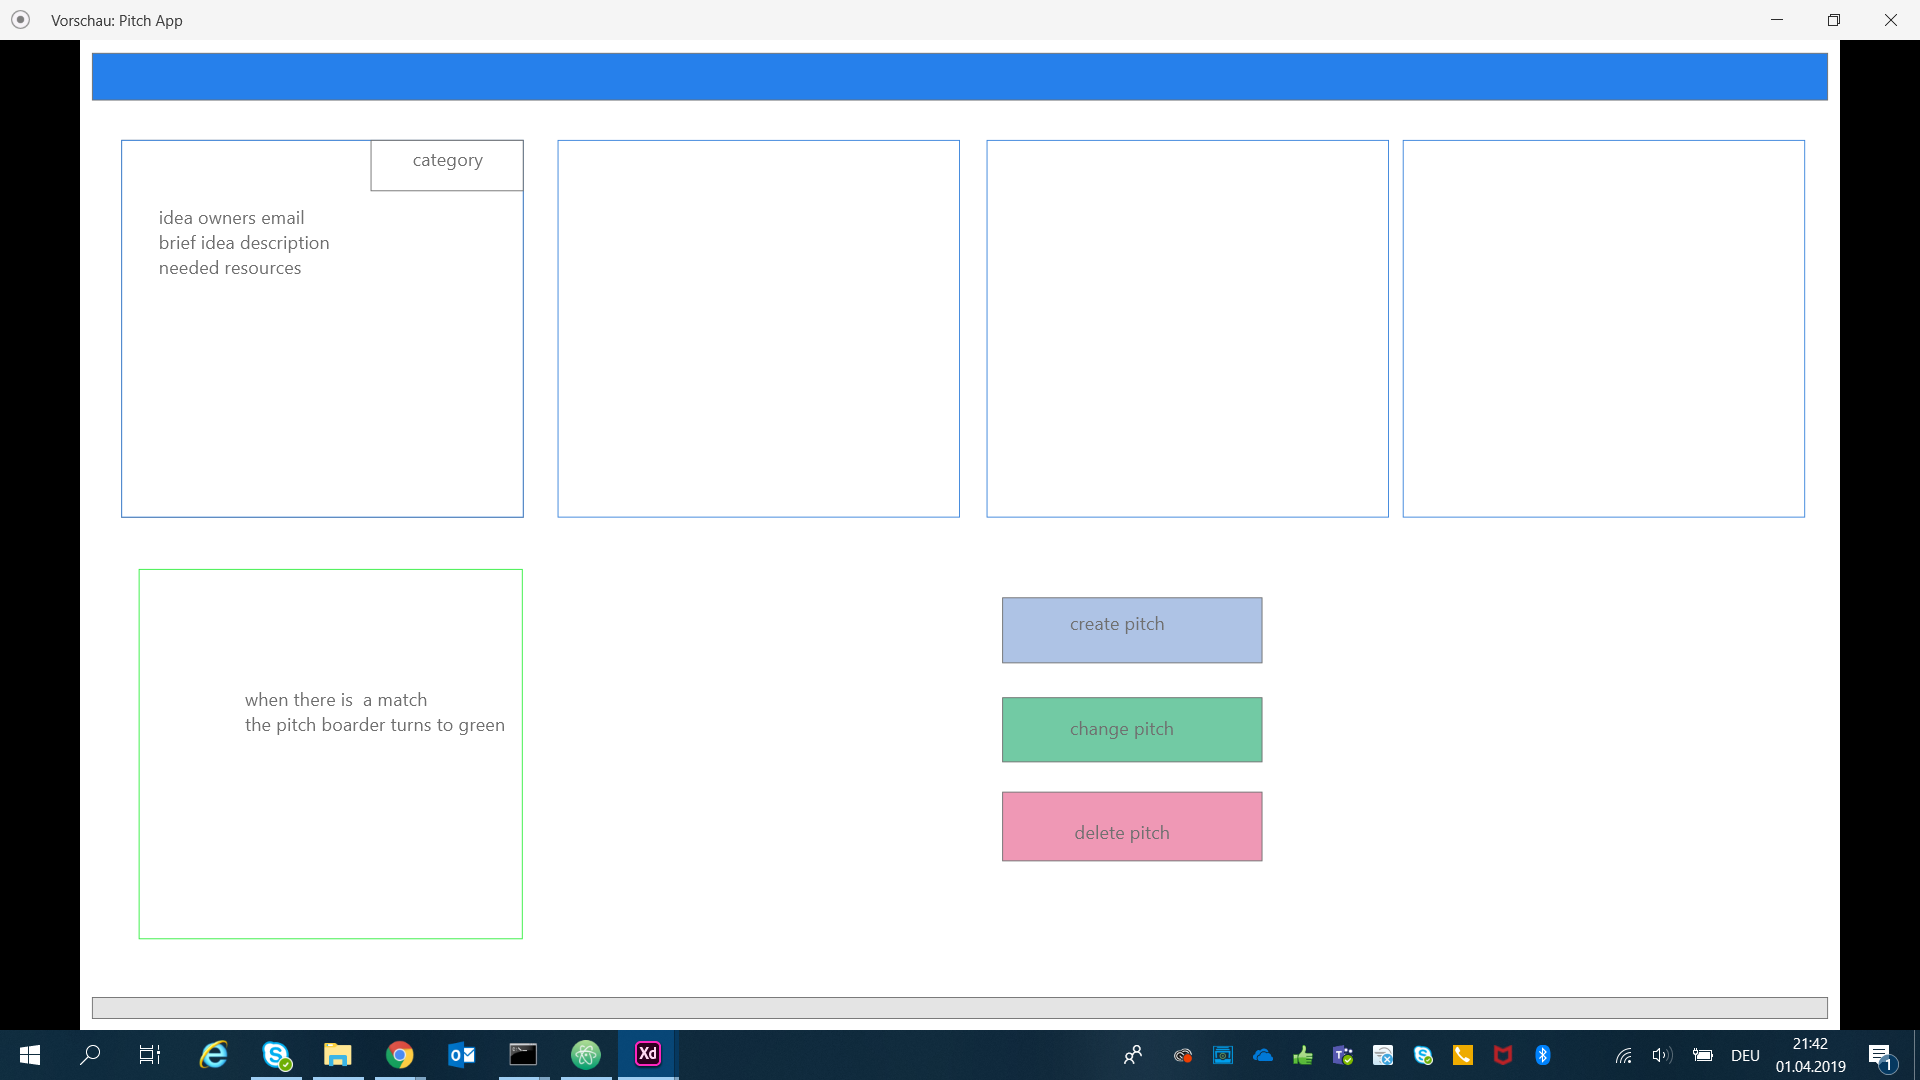
\includegraphics{home.png}
\end{center} 

Instead of designing the appearance of our own UI elements, which would cost us high effort, we were enabled to use already designed component-templates from Reactstrap \parencite{Reactstrap_comp}, combine them and - as a result - get a complex, yet neat looking UI design. In this way, we only had to decide how we combine these component-templates to create our own Reactstrap components. Our goal was to represent the users an intuitive UI. Furthermore, PitchApp was developed to be an "idea pool", where ideas of users must be very straightforward to collect and display. We also needed a simple way to represent states of Pitches, i.e. if a Match occurred to a Pitch. A Match means that an idea sponsor found that a posted idea (Pitch) is worth to be realized. This problem is also solved component-based. Each component manages states internally, which facilitated the handling of different states of UI elements. A render() method is implemented in each of the React components. This method takes input data and returns what to display. Render() can access input data by the attribute named "this.props". Internal state of a component can be accessed similarly with "this.state". Our goal was to build a convenient UI, where employees share their ideas happily and managers can smoothly brows between these. We used - inter alia - the Reactstrap components Badge to indicate a Match, Buttons to enable user interaction by clicking to navigate inside PitchApp, Jumbotron for an attractive landing page design, Media to include our logo and Modals to display additional information to the users.

React is compatible with Node, which we have also used on the server side for our back-end implementation. In other words, Node.js is a runtime environment for JS, with which React code can also be compiled.

An other advantage of React, that it is secure. By programming in JSX, it is safe to embed user inputs. React DOM escapes values coded in JSX before rendering them and all input is converted to string before rendering \parencite{JSX}. In this way, protection against injection attacks, especially against cross-site-scripting, is provided.

Additionally, Bootstrap \parencite{Bootstrap} should be mentioned, because Reactstrap component-templates are based on Bootstrap 4. Using the Bootstrap 4 layout grid system (more information can be found on \parencite{Bootstrap_grid}) facilitated the creation of a responsive UI, which was an explicit requirement for PitchApp. For this reason, Pitch App follows the principles of responsive web-design, which means that our web-application can be used on various sizes of screens including mobile phones and tablets. The UI components of PitchApp are able to automatically resize and move to display a nice-looking view on all kind of devices or window-sizes.

The following figures show how a full window-size version and a small window-size version of PitchApp's UI look with the reorganized UI elements.

\begin{center}
	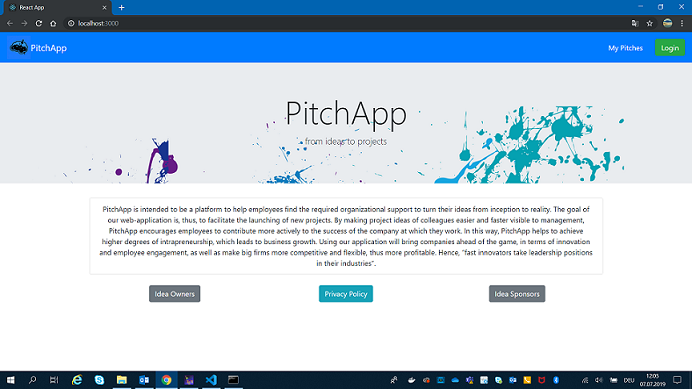
\includegraphics{pitchapp_big.png}
\end{center} 

\begin{center}
	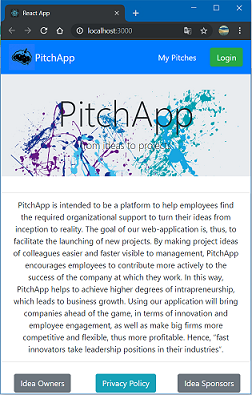
\includegraphics{pitchapp_small.png}
\end{center} 

During the design phase of PitchApp, our team decided to construct PitchApp to be a single-page web-application to enhance user experience. A single-page web-application intends to mimic the advantage of a desktop application and to avoid the unnecessary interruption of the user by saving navigation effort and time. The underlying idea is that, instead of loading whole page content repeatedly to the screen, only the changes are rendered. React adopts the principles of developing single-page applications, which was another argument for using React to the development of PitchApp. We used React routing components, like Router, Route, Redirect and History for managing session history, to achieve single-page rendering in PitchApp's App.js. Detailed explanation of different routing components with React can be found on reacttraining.com \parencite{React_router}.

To sum up, we can state that PitchApp was developed by using React and Reactstrap to be:

\begin{itemize}
	\item interactive,
	\item intuitive,
	\item secure,
	\item compatible,
	\item combinable,
	\item attractive,
	\item simple,
	\item single-page,
	\item responsive and
	\item dynamic.
\end{itemize}

\section{Okta Authentication}
\chapterauthor{by Ethan Kelly}

The User Management, Authentication \& Authorization along with Session Management for PitchApp is handled using the Okta Identity and Access Management Platform. Okta was chosen on the basis that it is fully OAuth 2.0 compliant, fully scalable and architected for zero downtime. Okta also offer many tools and services to help us with compliance and data security which we will discuss in the coming sections.

\subsection{Identity and Access Management (IAM)}

Identity and Access Management (IAM) are the framework of policies and technologies that ensure the proper people in an enterprise have the appropriate access to technology resources. Identity management can involve 4 basic functions:

\begin{itemize}
	\item Pure Identity – In all practical models of digital identity, a given identity object consists of a finite set of properties (attribute values). These properties record information about the object. A "pure identity" model is strictly not concerned with the external semantics of these properties.
	\item User Access - User access enables users to assume a specific digital identity across applications, which enables access controls to be assigned and evaluated against this identity. Access management is normally the motivation for identity management.
	\item Services - Many products require identity management to properly provide their services as they often require access to extensive information about a user which is subject to privacy and/or confidentiality requirements.
	\item Identity Federation - Identity federation comprises one or more systems that federate user access and allow users to log in based on authenticating against one of the systems participating in the federation. This trust between several systems is often known as "Circle of Trust". When a user needs to access some service controlled by SP, he/she first authenticates against the IdP and if successful an assertion is sent to the Service Provider.
\end{itemize}

Along with the capability to create, modify and delete identity data, Identity Management systems control data access and use across systems. To do this the system should have the following capabilities:

\begin{itemize}
	\item Authentication – Is the verification of if a user is who they say they are
	\item Authorization – Means managing what operations a user can execute.
	\item Roles – Roles are groups of operations or other roles which relate to a user’s job/tasks.
	\item Delegation – Delegation is the ability to allow another user to carry out tasks on your behalf.
	\item Interchange – The system needs a way of exchanging identity information across systems. The SAML and OpenID Connect protocols are common examples of such methods.
\end{itemize}

\subsection{The Shared Security Responsibility Model}

Okta makes use of the shared security responsibility model, a model used by many cloud providers including Amazon AWS and Microsoft Azure. This model specifies the distinct responsibilities of us (the customer) and the cloud provider.

\textbf{Okta's Responsibility}

Okta is responsible for the security of the Okta Identity Cloud Platform and its underlying infrastructure. They also provide features to allow us to fulfill our responsibilities.

\textbf{Our Responsibility}

We are responsible for securing our application using the features that Okta offer. This includes granting the correct permissions to users, protecting the right areas of the application and its data to ensure only authorized users see this information.

\begin{center}
	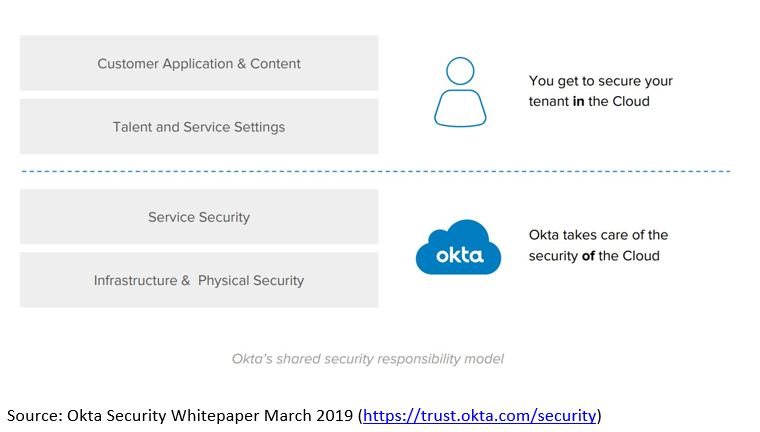
\includegraphics{okta1.png}
\end{center}

\subsection{Authentication and Authorization}

\textbf{Authentication}

As mentioned earlier, authentication is the process to verify if a user is who they say they are. Okta handles authentication for PitchApp. When users click Login within PitchApp they are forwarded to our Okta login page. Here users are given the opportunity to enter their login details, or when they are new and wish to register, they can use the provided form to create a user. The user will then receive an email to confirm their email address and registration. After successful registration the user is returned to PitchApp. When Okta redirects the user back to PitchApp it provides an authorization code and a user context that can be used within the app.

\textbf{Authorization}

PitchApp will then use this authorization code along with the required scope to request an access token from Okta. If the user is authorized to use such a scope an access token is returned. This token is then used when the user tries to use a restricted functionality of PitchApp, for example, sponsoring a Pitch. These tokens are also used by PitchApp to ensure users are only able to see information or Pitches, which they are authorized to see.
Okta works with Role-based Access Control which allows us to provide our customers with an even more personalized experience, while maintaining the upmost level of data security. Okta is also fully OAuth 2.0 compliant, this allows us to easily make use of the Role-based Access Controls, revoke access, and manage the token lifestyle. OAuth 2.0 is the industry standard protocol for authorization. It allows a user to gain limited access to a HTTP service.

\begin{center}
	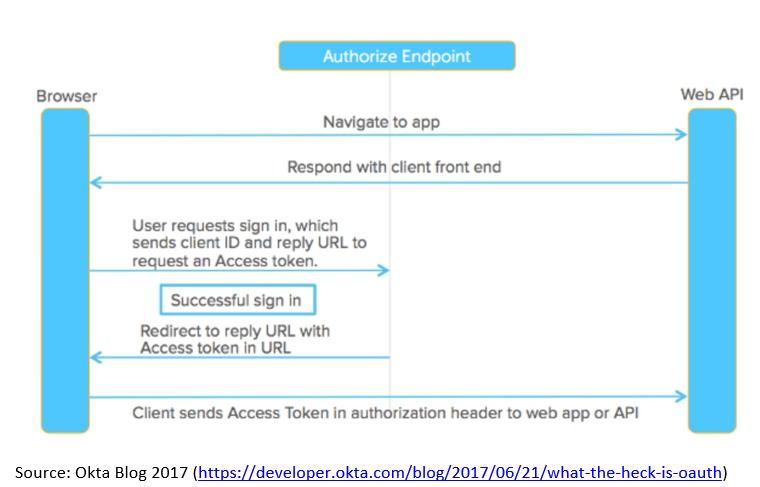
\includegraphics{okta2.png}
\end{center}

\subsection{Session Management}

A web session is a series of HTTP requests and responses created by the same user and session management is the set of rules that governs interactions between websites and its users. Sessions are established at a certain point in time, usually at the time of authentication, and torn down usually at the time of logout or after a timeout. There are 2 forms of session management, cookie-based and URL-rewriting.
Okta uses a cookie-based authentication mechanism to maintain a user's authentication session across web requests. Session cookies have an expiration configurable by an administrator for the organization and are valid until the cookie expires or the user closes the session (logout) or browser application. A session token is returned after successful authentication which can be later exchanged for a session cookie. Encrypted connections are used for all communications with Okta.

\section{GraphQL Hasura Engine as Server}
\chapterauthor{by Csaba Kegyes}
\section{PostgreSQL Database}
\chapterauthor{by Csaba Kegyes}
\section{Docker}
\chapterauthor{by Csaba Kegyes}
\chapter{Final Results}
\chapterauthor{by Stella Kamakari}
\chapter{User Manual}
\chapterauthor{by Stella Kamakari}
\chapter{Difficulties of Implementation}
\section{Difficulty 1}
\chapterauthor{by Boglarka Lehoczki}
\section{Difficulty 2}
\chapterauthor{by Csaba Kegyes}
\section{Difficulty 3}
\chapterauthor{by Stella Kamakari}
\section{Difficulty 4}
\chapterauthor{by Ethan Kelly}
\chapter{Future Outlook: Missing Components and Functionalities}
\chapterauthor{by Stella Kamakari}



